\chapter{The Top Quark}
\label{Chapter:TheTopQuark}
%\addcontentsline{toc}{chapter}{The Top Quark}

\section{The Standard Model}

\begin{itemize}

\item Intoduction to the SM of particle physics, model used to explain all observed phenomena at the particle level, with the exception of gravity and large scale cosmological things like Dark Matter and Dark Energy.

\item It is a guage theory where interactions due to fundamental forces are modelled by exchange particles called bososn. 

\item Explain grouping of fermions into generations. Explain quarks and leptons.

\item $SU(3)_{colour}$ associated with colour charge and has eight guage bosons called "gluons". All observable objects are colourless i.e. neutral colour charge. Physical interactions solely governed by the strong force are know as QCD.

\item $SU(2)_{isospin} x U(1)_{hypercharge}$ assoicated with isospin and hypercharge. Physical interactions goverend by the Electroweak force are known as QCD. It's bosons are massless photons and W, Z bosons.

\item What about Higgs?

\item Maybe explain about V-A interactions?

\end{itemize}

%\section{The Heaviest Particle}
%Mention Higgs role in giving fermions mass and that the top quark is the same size as an Itrium atom (or perhaps more relatably, the gold atom) and yet is point like. Explain how it was predicted from SM EW fits that the top mass would be in a range of 140\GeV to 180\GeV, and yet this is still only a constraint based of multiparameter fits, and there remains no reason for the top quark mass to be so much heavier than the other fermions and bosons. (Maybe say something about how it may play a role in EW symmetry breaking.

\section{Strong Production of Top Quark Pairs}
\ttbar\ pair production occurs via two primary channels at hadron colliders, fusion of two gluons or anihilation of two quarks. Production via lepton fusion is possible though no lepton collider has yet been constructed with the necessary centre of mass energy. The leading order production diagrams are shown in figure \ref{fig:ttbar_prod}.

\begin{itemize}
  \item s-channel, t-channel, u-channel production.
  \item gluon gluon dominated at LHC
  \item q qbar from sea quarks
  \item assymetries
\end{itemize}

\section{Top Quark Decay}

\begin{itemize}
  \item $|V_{tb}|$
  \item classification of decay channel
  \item V-A structure
\end{itemize}

\section{Spin Correlations}

\subsection{Definition}
Spin correlation is the degree to which the spin information of one top quark is coupled to another. If the spins of a top and anti-top quark were fully correlated then knowing the spin of one quark would be sufficient to extrapolate the spin of the other quark. 

Top quark production is a QCD process and as such is invariant under parity transformations. In the SM case we would expect that the top quark has no intrinsic polarisation arising from QCD~\cite{NOQCDPOLARISATION}. That is we could not say for sure what the direction of spin a top quark has based on it's direction of momentum. A degree of polarisation is possible due to electroweak interactions, but contributions of this nature are expected to be very small~\cite{EWPOLARISATIONSMALL}. We cannot make a definitive statement on top quark spin direction or anti-top quark spin direction alone, however we can investigate the degree to which these directions are correlated.

Spin correlation is the degree to which the spin information of one top quark is coupled to another. If the spins of a top and anti-top quark were fully correlated then knowing the spin of one quark would be sufficient to extrapolate the spin of the other quark. In practice we may define a ratio of the number of events where the spins of the top and anti-top are aligned and the number of events where the spins are anti-aligned:
%%%%% EQUATION %%%%%
\begin{equation}
    A = \frac{N_{like} - N_{unlike}}{N_{like} + N_{unlike}} =
     \frac{N(\uparrow \uparrow) + N(\downarrow \downarrow) - N(\uparrow \downarrow) - N(\downarrow \uparrow)}
     {N(\uparrow \uparrow) + N(\downarrow \downarrow) + N(\uparrow \downarrow) + N(\downarrow \uparrow)}.
    \label{eq:Adef}
\end{equation}
%%%%%%%%%%%%%%%%%%%
The purpose of this thesis is to measure this parameter A and to determine to what degree, if any, the top quark spin and anti-top quark spins are correlated. 

\subsection{Accessing spin correlations via angular distributions}

The spin information for the top quark can be accessed through the angular distributions of its decay particles. Equation \ref{equ:topdiffxsec} shows the differential cross section for \ttbar\ production:
%%%%% EQUATION %%%%%
\begin{equation}
\frac{1}{N} \frac{dN}{d \cos (\theta_i)} = \frac{1}{2} \left[1 + P \alpha_i \cos(\theta_i) \right],
\label{equ:topdiffxsec}
\end{equation}
%%%%%%%%%%%%%%%%%%%
where $\theta_i$ is the angle of the charged lepton relative to a spin axis in the parent top rest frame, P is the polarisation of the top, and $\alpha_{i/j}$ is the spin analysing power of the lepton. We can then define the double differential cross section:
\begin{equation}
\frac{1}{\sigma} \frac{d\sigma}{d\cos\theta_+ d\cos\theta_-} =
\frac{1}{4} ( 1 - C \cos\theta_+ \cos\theta_- ) \,\, ,
\label{eq:coscos}
\end{equation}
where in the SM case the polarisation parameter, P, is very small in accordance with the SM expectation and with results from other ATLAS analyses~\cite{polarisation}. $\sigma$ denotes the cross section of the channel under consideration. $\theta_+$ ($\theta_-$) describes the angle between the direction of flight of the lepton $\ell^+$ ($\ell'^-$) in the $t$($\bar{t}$) rest frame and a reference direction $\bf \hat{a}$ ($\bf\hat{b}$). The choice of this reference direction ("spin basis") determines the extent to which the spins of the top quarks are correlated. $C$ is a free parameter between -1 and 1 that depends on the choice of the spin basis and is defined as the amount of observable spin correlation (A) multiplied by the spin analysing power ($\alpha_{i/j}$) of the particles used to measure the $\theta^{+/-}$ angles:
%%%%% EQUATION %%%%%
\begin{equation}
    C = \alpha_{i}*\alpha_{j}*A.
\end{equation}
%%%%%%%%%%%%%%%%%%%

An important quantity to consider how much of the spin information from the \ttbar\ pair may be accessed via the decay particles. Table~\ref{tab:alphas} shows the spin analysing power of each particle in the \ttbar\ decay for a top quark mass ($m_t$) of 172.5 GeV . The charged leptons coming from the W boson decay carry the full spin information of the parent top quarks at LO, and hence observables constructed with the charged leptons in the dilepton channel have the highest sensitivity. The down type quark originating from the W decay also has high spin analysing power, however these are difficult to differentiate from the less sensitive up type jet from the same W, and hence the semi-leptonic channel loses some sensitivity. In previous results from the Tevatron, the principal disadvantage of the dilepton channel was limited statistics. The dilepton channel's branching ratio is only 20\% that of the semi-leptonic channel however this is no longer a limiting factor due to the large statistics available at the LHC. The dilepton channel is therefore the most sensitive channel for spin correlation analyses. 

\begin{table}[htbp]
\begin{center}
\begin{tabular}{|c||c|c||c||c|c|}
\hline
                 & $b$-quark & $W^+$ & $l^+$ & $\bar{d}$-quark or $\bar{s}$-quark& $u$-quark or $c$-quark\\
\hline
$\alpha_i$ (LO)  & -0.410    & 0.410 & 1.000 & 1.000                             & -0.310 \\
$\alpha_i$ (NLO) & -0.390    & 0.390 & 0.998 & 0.930                             & -0.310 \\
\hline
\end{tabular}
\end{center}
\caption{Standard Model spin analysing power, at leading order and next-to-leading order for the decay products of the top quark (with a mass of 172.5 GeV ) from the decay $t \ra bW^+$.  The decay products of the $W$-boson can also be used as spin analysers, hence the decay products from leptonic decays $W^+ \ra l^+\nu_l$ and the hadronic decays $W \ra q_1\bar{q}_2$ are also given in the table. These values are for top quark with particular spin direction, the signs are reversed for a top quark with opposite spin~\cite{hubaut, Czarnecki:1990pe, Brandenburg:2002xr}.}
\label{tab:alphas}
\end{table}

\subsection{Spin analysing basis}
\label{sec:spinanalysingbasis}
In order to measure the spin correlation it is necessary to define a reference basis from which we will derive the spin direction. This choice is not trivial and can greatly effect the amount of observable spin correlation. Thusfar we have discussed the spin direction in terms of the top qaurk momentum direction, hereafter referred to as the \emph{``Helicity"} basis but there are additional bases from which we may choose to make a measurement. In the simplest case we may use the beamline as a reference basis. In previous studies at the Tevatron, the beamline basis was an effective basis to choose with a high degree of observable spin correlation~\cite{TEVATRONSPIN,BEAMLINE DESCRIPTION}. In the case of a $p$-$\bar{p}$ collider, such as the Tevatron, the beamline approximates the direction for the incoming proton and anti-proton and hence the incoming quark and anti-quark that dominate \ttbar\ production have a high momentum fraction in this direction. At the LHC one of the quarks must come from the sea and this basis no longer approximates the direction of one of the incoming quarks.


At leading order (LO), production of \ttbar\ pairs at the LHC may occur via two channels; gluon fusion and $q\bar{q}$ anihilation. If the initial spin structure is also considered this leads to three possible production states:
\begin{enumerate}
\item $q_\mathbf{L}\bar{q}_\mathbf{R}$ and $q_\mathbf{R}\bar{q}_\mathbf{L}$: Opposite helicity quark anti-quark annihilation.
\item g$_\mathbf{L}$g$_\mathbf{R}$ and g$_\mathbf{R}$g$_\mathbf{L}$ : Opposite helicity gluon fusion.
\item g$_\mathbf{L}$g$_\mathbf{L}$ and g$_\mathbf{R}$g$_\mathbf{R}$ : Like helicity gluon fusion.
\end{enumerate}
Production can occur between threshold ($\beta \rightarrow 0$) and the ultra high relativistic limit ($\beta \rightarrow 1$). No variable exists that is maximally sensitive to all initial spin configurations and production boosts so we investigate a number of variables, each differently sensitive to the initial spin state. It can be shown that, for the purposes of spin correlation, initial state (1) and (2) are equivalent~\cite{mahlon:2010}. 

\ttbar\ production at the LHC is dominated by gluon fusion, with only small contributions from $q\bar{q}$ annihilation. The ratio of like helicity to unlike helicity gluons is approximately 65\% vs 35\%~\cite{mahlon:2010} and it is advantageous to exploit variables sensitive to like helicity gluon fusion.Two such variables exist, the ``S-Ratio" and $\Delta\phi$ variable. The S-Ratio~\cite{mahlon:2010} is defined in equation \ref{eq:sratio} as the ratio of correlated and uncorrelated matrix elements in the helicity basis~\cite{mahlon:2010}:
%%%%%%%% EQUATION %%%%%%%
\begin{equation}
  S = \frac{(|A|_{\mathbf{RR}}^2 + |A|_{\mathbf{LL}}^2)_{corr}}{(|A|_{\mathbf{RR}}^2 + |A|_{\mathbf{LL}}^2)_{uncorr}}= \frac{m_t^2\{(t \cdot l^{+}) * (t \cdot l^{-}) + (\tbar \cdot l^{+}) * (\tbar \cdot l^{-}) - m_t^2 * (l^{+} \cdot l^{-})\}}
           {(t \cdot l^{+})*(\tbar \cdot l^{-})*(t \cdot \tbar) }.
\label{eq:sratio}
\end{equation}
%%%%%%%%%%%%%%%%%%%%%%%%
At low $\beta$, S is maximal when the charged leptons are parallel and at a minimum when they are back to back. As $\beta$ increases this remains true but the lepton momenta become correlated with the top anti-top spin axis. The charged leptons are more likely to be parallel than back to back in the LL or RR configuration. At low \ttbar\ invariant mass this manifests in the $\Delta\phi$ as a suppression in low values of $\Delta\phi$ and enhancement of high $\Delta\phi$ when compared to the uncorrelated case, illustrated in Fig.~\ref{fig:parton_dphi}. This same effect is seen in the S-Ratio distributions in Fig.~\ref{fig:parton_sratio} however in this case the values for the S-Ratio are enhanced closer to one and supressed at low values relative to the uncorrelated spin case. At high values for invariant mass (close to the relativistic limit $\beta \rightarrow 1$) this is no longer the case and the percentage of like helicity gluons are reduced, resulting in diminished separation between the correlated and uncorrelated case.

At high values of \ttbar\ invariant mass, production occurs at high $\beta$ and has an enhanced contribution from unlike helicity gluons and $q\bar{q}$ annihilation. The $\cos(\theta^+)\cos(\theta^-)$ variables exploited in previous Tevatron results are useful in this case~\cite{do_spin}. We define the $\cos(\theta^+)\cos(\theta^-)$ where $\theta$ is the angle between the charged lepton and some chosen basis in the zero momentum frame of the parent top quark.

For purely $q\bar{q}$ produced \ttbar\ pairs or for unlike helicity gluons the $\cos(\theta^+)\cos(\theta^-)$ variable where the angles are measured with respect to the top quark helicity in the top rest frame ("helicity basis") is most appropriate at the LHC. 

In addition, a different basis exists for which the observable spin correlation arrising from gluon-gluon fusion initial states (both oposite and like helicity) may be maximised, the \emph{maximal} basis. This basis is constructed by taking the largest eigenvector of the spin density matrix for gluon fusion production and is by definition the basis that is most sensitive to the observation of spin correlations arising from gluon gluon fusion~\cite{Uwer:2004vp}. 

Experimentally the $\cos(\theta^+)\cos(\theta^-)_{maximal}$ and S Ratio variables both require full event reconstruction which is susceptible to mismodelling and combinatorics effects, whereas the $\Delta\phi$ variable is observable in the lab frame and hence has the highest experimental sensitivity. 
\newline
\newline
In summary four variables are studied:
\begin{enumerate}
\item $\Delta\phi$: A lab frame variable highly sensitive to spin correlations arising from like helicity gluon production. This variable is well motivated in both the inclusive selection and at low values of reconstructed \ttbar\ invariant mass, but it is also studied in the low and high invariant mass regimes.
\item S-Ratio\cite{mahlon:2010}: A reconstruction level variable sensitive to like helicity gluon production at low invariant mass. As this variable is a ratio some systematics effects may be mitigated. 
\item $\cos(\theta^+)\cos(\theta^-)_{helicity}$: A reconstruction level variable and the only variable directly sensitive to unlike helicity initial states over the entire invariant mass range, though it is also investigate in all mass regimes. This is the only variable that is sensitive to contributions from the $q\bar{q}$ initial state.
\item $\cos(\theta^+)\cos(\theta^-)_{maximal}$~\cite{Uwer:2004vp}: A reconstruction variable sensitive to production from gluon fusion in general (both like helicity and oposite helicity) and theoretically the maximally sensitive variable to spin correlations, though this is suppressed to a degree by reconstruction effects. It is measured in the inclusive, high and low mass regimes.
\end{enumerate}

\subsection{Correlation between variables}

All of the analysis variables measure spin correlation however they are differently sensitive to spin correlations arising from different initial helicity states. It is therefore useful to investigate the correlation between the analysis variables. The correlation was estimated by performing the fit described in section \ref{sec:extraction}, simultaneously for each variable using ensemble tests generated from MC. The correlations investigated at reconstruction level are shown in Fig.~\ref{fig:correlation} and listed in Table~\ref{tab:correlations}. The degree to which each variable correlated to another varies depending on the overlap in sensitivity to the initial spin state and production mechanism. For example it is expected that the Helicity and Maximal basis have a high degree of correlation, though the helicity basis has some sensitivity to production via quark anti-quark annihilation unlike the Maximal basis which is formulated to be maximally sensitive to spin correlations arising from gluon gluon fusion.

\begin{table}[htbp]
\begin{center}
\begin{tabular}{c | c c c c }
	                   & $\mathbf{\Delta\phi} $ & \textbf{Helicity} & \textbf{Maximal} & \textbf{S Ratio} \\
\hline
$\mathbf{\Delta\phi} $ &       & 0.313 & 0.353 & 0.616 \\
\textbf{Helicity}      & 0.313 &       & 0.682 & 0.646 \\
\textbf{Maximal}       & 0.353 & 0.683 &       & 0.552 \\
\textbf{S Ratio}       & 0.616 & 0.646 & 0.552 &       \\
	
\end{tabular}
\end{center}
\caption{Table of correlations between analysis variables at reconstruction level, measured with $10^5$ ensemble tests.}
\label{tab:correlations}
\end{table}

\begin{figure}[htpb!]
\begin{center}
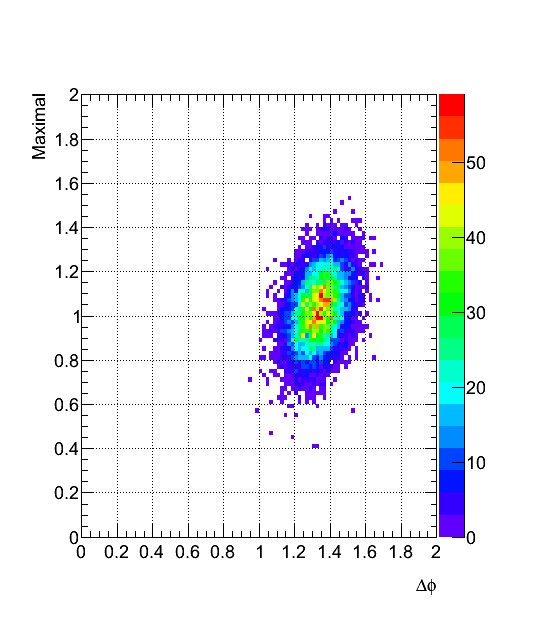
\includegraphics[width=75mm]{f/correlation_dphi_op}
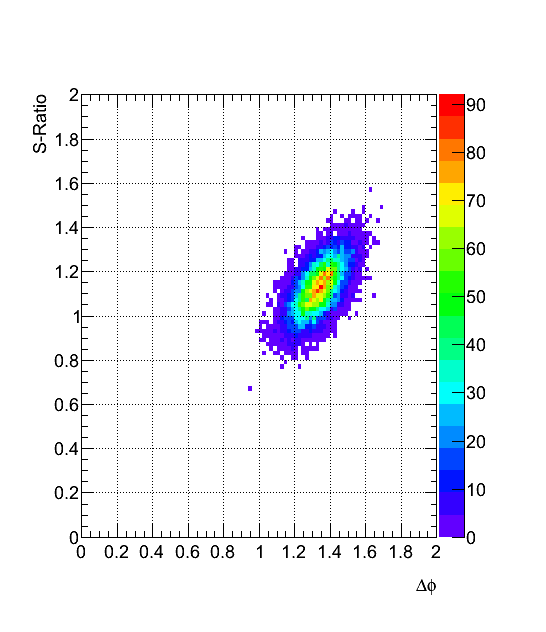
\includegraphics[width=75mm]{f/correlation_dphi_sratio}
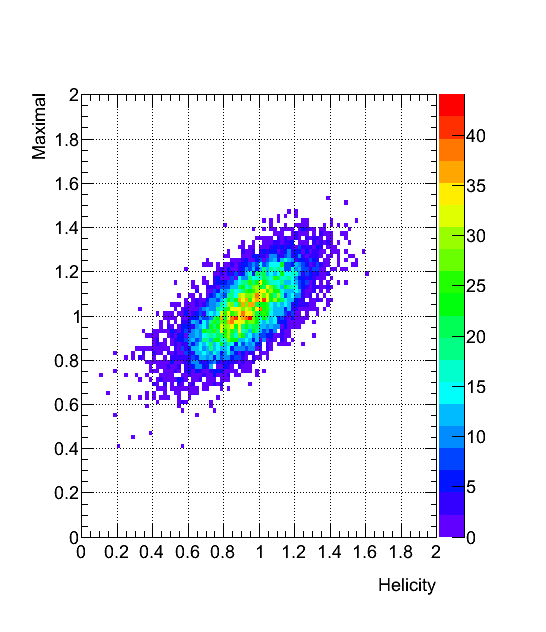
\includegraphics[width=75mm]{f/correlation_hb_op}
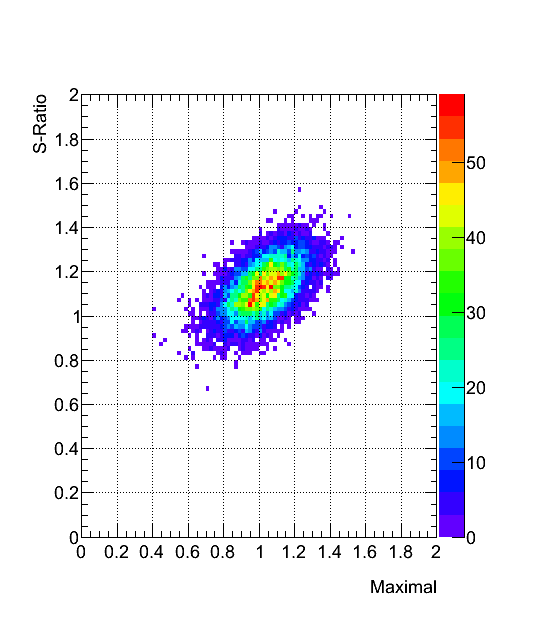
\includegraphics[width=75mm]{f/correlation_op_sratio}
\end{center}
\caption{Correlation between the analysis variables after event reconstruction and selection. The correlation displayed is between the extracted fraction of SM like spin correlation (described in section~\ref{sec:extraction}) for each variable. A low degree of correlation is observed between $\Delta\phi$ and the cosine variables. As a cross check the correlation between two similar cosine variables (helicity and maximal) is measured. A high degree of correlation is observed as expected.}
\label{fig:correlation}
\end{figure} 

\begin{figure}[htpb!]
\begin{center}
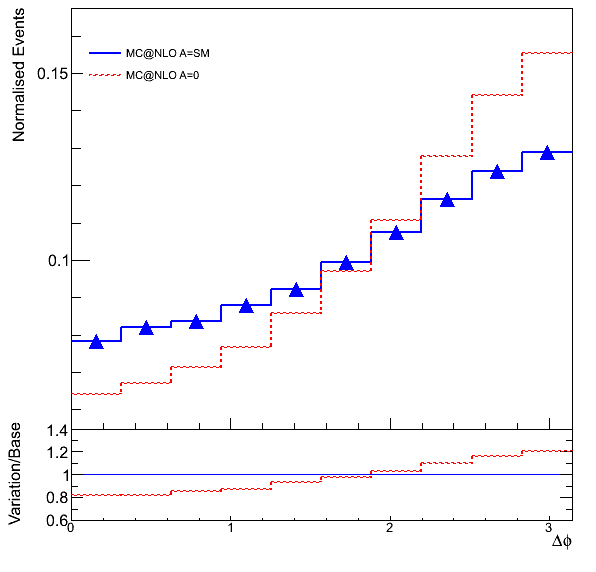
\includegraphics[width=52mm]{f/truth_delta_Phi10_truth_comparison}
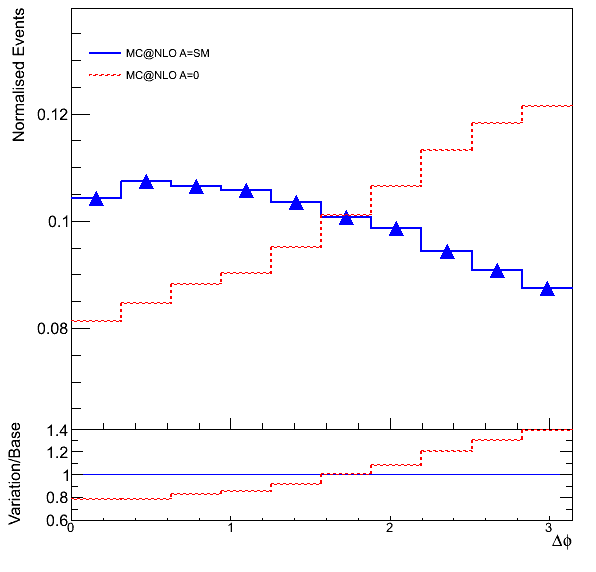
\includegraphics[width=52mm]{f/truth_delta_Phi10_low_truth_comparison}
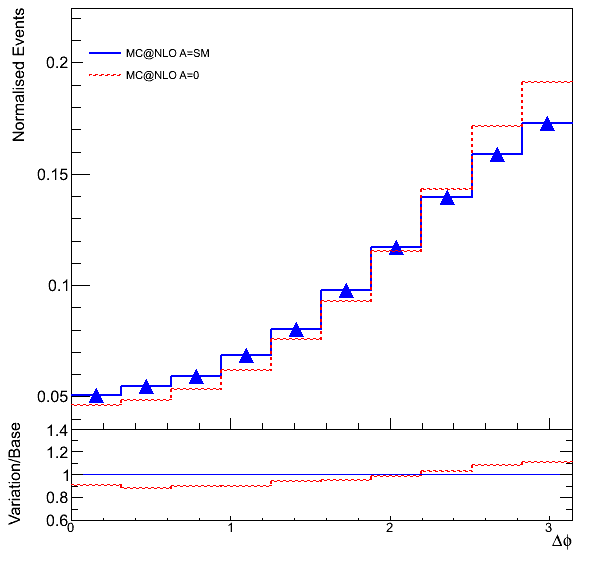
\includegraphics[width=52mm]{f/truth_delta_Phi10_high_truth_comparison}
\end{center}
\caption{Distribution of \dphi\ for parton level MC@NLO events at $\sqrt{s}=7$~TeV for all events (left), for events with \ttbar\ invariant mass less than 450 GeV (center) and invariant mass higher than 450 GeV (right). The histogram shows the Standard Model and uncorrelated scenarios. }
\label{fig:parton_dphi}
\end{figure} 

\begin{figure}[htpb!]
\begin{center}
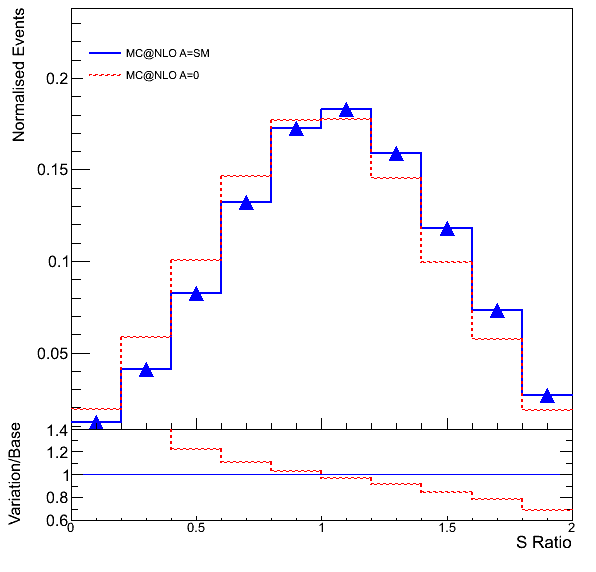
\includegraphics[width=52mm]{f/truth_rratio_truth_comparison}
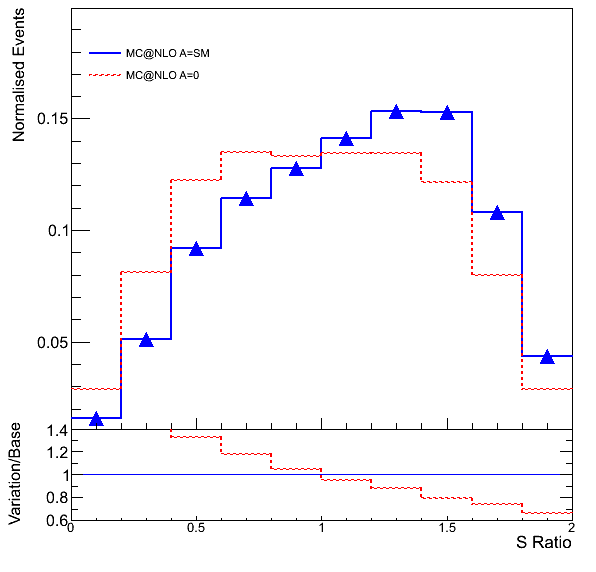
\includegraphics[width=52mm]{f/truth_rratio_low_truth_comparison}
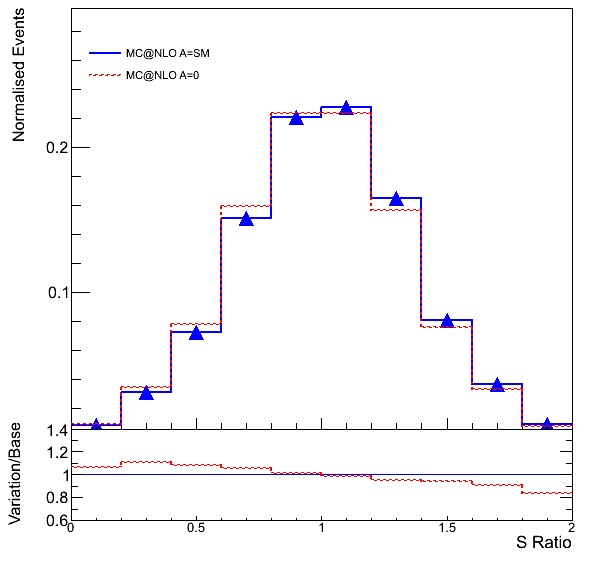
\includegraphics[width=52mm]{f/truth_rratio_high_truth_comparison}
\end{center}
\caption{Distribution of S-Ratio for parton level MC@NLO events at $\sqrt{s}=7$~TeV for all events (left), for events with \ttbar\ invariant mass less than 450 GeV (center) and invariant mass higher than 450 GeV (right). The histogram shows the Standard Model and uncorrelated scenarios. }
\label{fig:parton_sratio}
\end{figure} 

\begin{figure}[htpb!]
\begin{center}
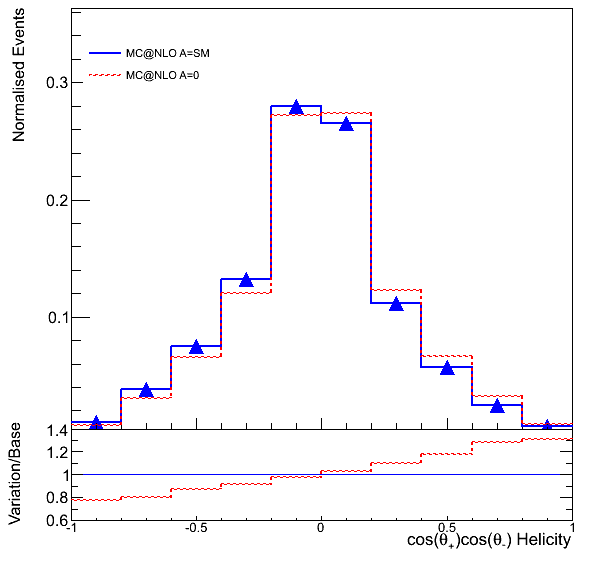
\includegraphics[width=52mm]{f/truth_coscos_hb_truth_comparison}
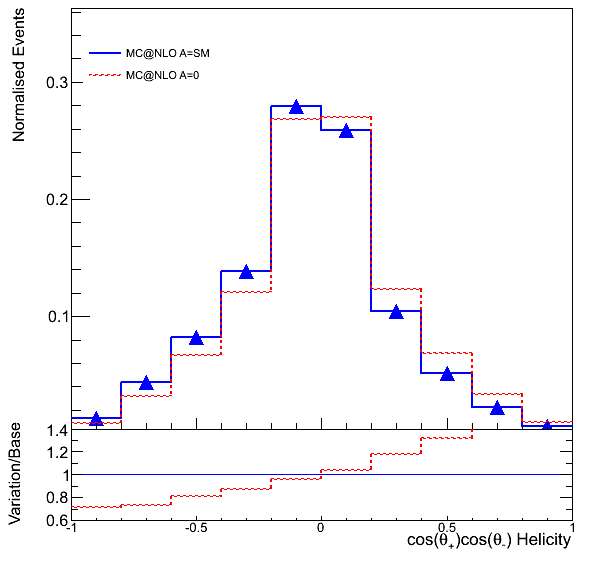
\includegraphics[width=52mm]{f/truth_coscos_hb_low_truth_comparison}
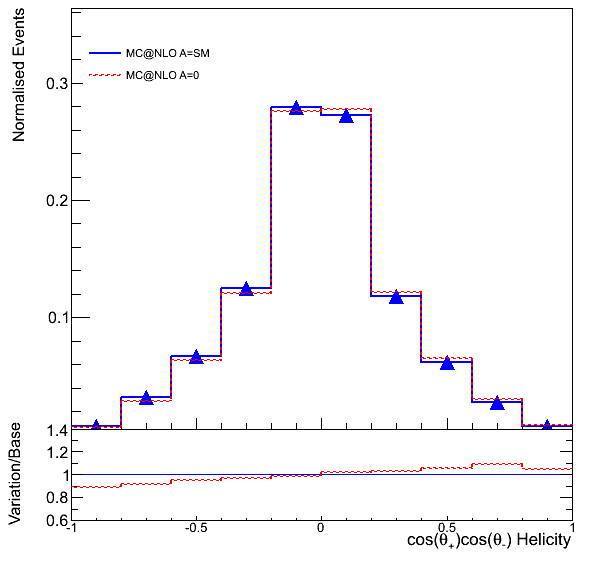
\includegraphics[width=52mm]{f/truth_coscos_hb_high_truth_comparison}
\end{center}
\caption{Distribution of $cos(\theta^{+})cos(\theta^{-})_{HELICITY}~$ for parton level MC@NLO events at $\sqrt{s}=7$~TeV for all events (left), for events with \ttbar\ invariant mass less than 450 GeV (center) and invariant mass higher than 450 GeV (right). The histograms shows the Standard Model and uncorrelated scenarios. }
\label{fig:coscoshb}
\end{figure} 

\begin{figure}[htpb!]
\begin{center}
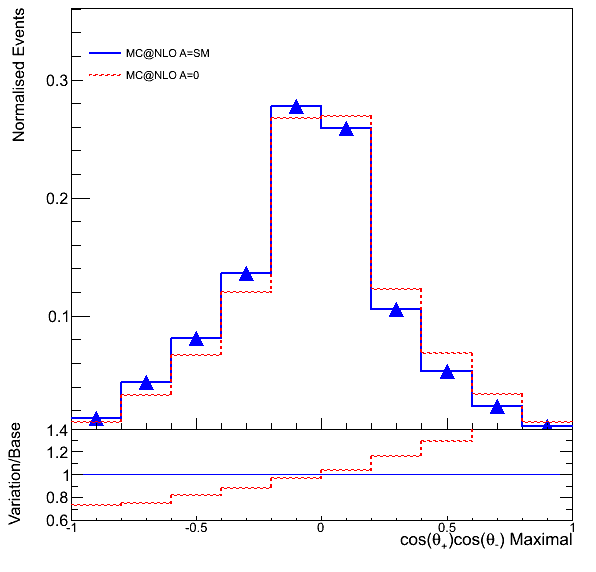
\includegraphics[width=52mm]{f/truth_coscos_op_truth_comparison}
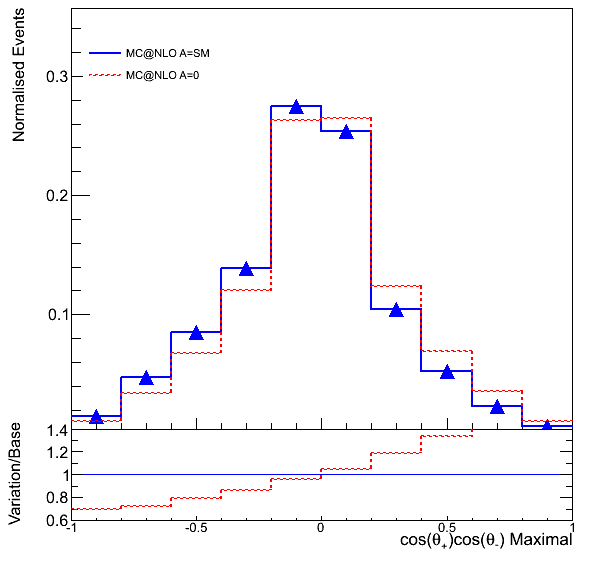
\includegraphics[width=52mm]{f/truth_coscos_op_low_truth_comparison}
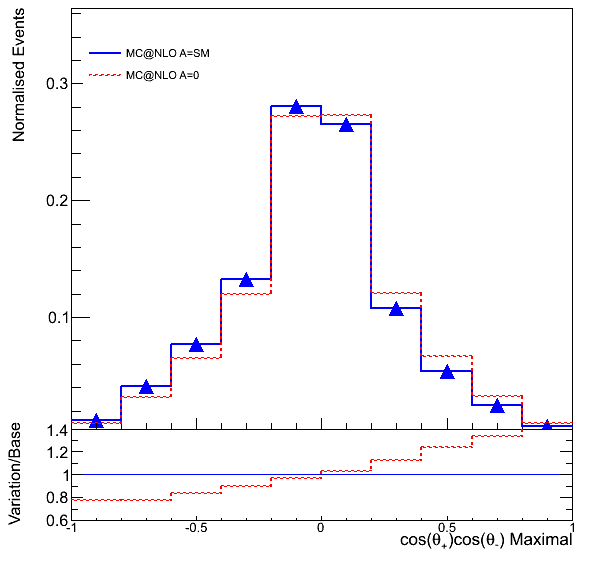
\includegraphics[width=52mm]{f/truth_coscos_op_high_truth_comparison}
\end{center}
\caption{Distribution of $cos(\theta^{+})cos(\theta^{-})_{MAXIMAL}~$ for parton level MC@NLO events at $\sqrt{s}=7$~TeV for all events (left), for events with \ttbar\ invariant mass less than 450 GeV (center) and invariant mass higher than 450 GeV (right). The histograms shows the Standard Model and uncorrelated scenarios. }
\label{fig:coscos}
\end{figure} 

%\subsection{Like Helicity Gluons}
%\subsection{Oposite Helicity Gluons and Fermions}

\section{Probing Beyond The Standard Model}




